\chapter{相关研究现状}
并行软件技术主要跟随并行硬件的发展在发展,并且一直处于学术界与工业界热点关注之下。
并行软件技术种类繁多,根据不同的标准可以做不同的归类,
分类依据包括适用的硬件系统结构(共享内存与分布式内存)、
处理器类型(通用CPU与面向特定领域的协处理器)、
并行编程模型(消息传递与数据并行)等。
本章将介绍三类并行软件技术,
%% 本章以并行软件工具自身设计特点作为依据,将并行编程技术分为两类:并行程序库与
%% 并行程序语言,
第\ref{sec:parallel-library}介绍并行程序库技术,
并行程序库这是所有更高层并行软件技术的实现基础。
第\ref{sec:parallel-language}将介绍并行程序语言的研究现状,
由于本论文课题属于函数式并行程序语言研究,
将着重介绍函数式程序语言并行编程技术的研究现状。
%% 此外,鉴于异构系统的与协处理器的重要性,还将专门
%% 开辟第\ref{sec:gpu-parallel-prog}节介绍面向协处理器(主要是GPU)的并行编程技术。

\section{并行程序库技术}\label{sec:parallel-library}
并行程序库是基础的并行编程技术,一般作为系统软件提供给编程者使用。编程者可以直接
调用程序库中的API进行并行编程,也可以使用并行程序库实现更高级的并行编程工具,如
实现新的并行编程语言、开发并行编译器等。本节将介绍两类并行程序库,多线程技术应用
于共享内存计算机,消息传递接口MPI应用于分布式内存计算机。

\subsection{多线程技术}
多线程(multi-threading)技术是所有并行编程技术的实现基础,现有的并行编程技术基本
都要利用多线程技术才能实现。线程,在逻辑上是一个独立的指令序列,属于不同线程的
指令可以独立并行执行而互不干扰。多线程的概念源于多进程,同多进程一样,线程最初的设计
初衷是为了提高系统吞吐率,避免处理器因为某些耗时较大的操作(如读写磁盘)产生空转
浪费计算资源。所以,最初的多线程程序运行于单核心处理器,不同线程通过分时交替执行,
并非真正的并行执行。后来,随着多核处理器的出现,多线程程序可以真正并行地运行在
多个处理器核心之上。

多线程一般由操作系统提供支持,形式为一组C语言API,实现线程的创建、
回收、通信等功能,在当前的主流通用计算平台上都有实现,
如Windows的Win32线程\upcite{Cohen1998},
Linux的LinuxThreads\upcite{Leroy1996}与NPTL\upcite{Drepper2003}。
1995年IEEE发布了POSIX线程标准,称为Pthreads,Pthreads
规范了多线程程序库API设计,使得多线程程序具有更好的移植性。

多线程技术采用MIMD编程模型,非常适用于通用CPU的硬件结构,是对通用CPU硬件的直接抽象。
多线程技术对称序行为的控制能力强,性能高。但多线程技术抽象层次低,要求编程者显式地
控制所有并行细节,编程复杂度高,且可移植性差。总体上直接使用多线程技术的软件成本
较高。多线程技术只能技术应用于共享内存计算机。

\subsection{消息传递接口}
消息传递接口MPI是一个API规范\upcite{Geist1996},定义了一组用于在并行计算机上编写并行程序的消息传递API,
MPI也是一种编程模型,是对分布式内存计算机(尤其是由独立计算机通过网络
互联组成的计算机集群)的直接抽象。
MPI定义了运行于不同计算机的进程之间的通行行为,独立于具体程序语言与通信协议。
MPI也可以用于共享内存计算机,同样适用于定义线程间通信行为。

MPI的设计初衷是高性能、可扩展性、可移植性,长期以来,MPI在分布式内存计算机系统尤其是
大型计算机集群与超级计算机上表现十分优秀,一直是在大规模科学计算领域占据支配地位的
并行编程技术。同多线程模型一样,MPI编程模型的抽象层次低,细节隐藏能力差,编程复杂度
较高。

MPI定义了上百个API,但通常只需要使用其中6个就可以完成许多并行程序的编写,参见表\ref{tbl:mpi-api}。
\begin{table}
  \centering
  \caption{MPI常用API}
  \label{tbl:mpi-api}
  \begin{tabularx}{\linewidth}{lX}
    \toprule[1.5pt]
    \hei{API} & \hei{功能说明}\\
    \midrule[1pt]
    \texttt{MPI\_Init} & MPI初始化函数,必须先于所有其他MPI调用被调用\\
    \texttt{MPI\_Finalize} & MPI结束函数,必须在MPI程序结束前调用\\
    \texttt{MPI\_Comm\_rank} & 返回当前进程在给定通信域中的标识\\
    \texttt{MPI\_Comm\_size} & 返回给定通信域中的进程数\\
    \texttt{MPI\_Send} & 发送消息\\
    \texttt{MPI\_Recv} & 接收消息\\
    \bottomrule[1pt]
  \end{tabularx}
\end{table}

MPI有多个可用实现。Argonne国家实验室与Mississippi州立大学给出了MPI-1.x的第一个实现MPICH,
后来又开发了支持MPI-2.1的MPICH 2。OpenMPI是另一个广泛使用MPI实现,它吸收了若干个早期
MPI实现(FT-MPI, LA-MPI, LAM/MPI)的技术。此外,IBM、HP、Intel等厂商都提供了自己的
商业版MPI实现。

\section{函数式语言并行编程技术}\label{sec:parallel-language}
上一节介绍的两种并行程序库技术,分别是对共享内存计算机与分布式内存计算机硬件结构的直接
抽象,这两种并行编程技术对程序行为控制力强,但编程复杂度高。也就是说,并行程序库的方法
在高效性方面表现较好但在易用性方面仍显不足。

并行程序语言是解决易用性问题的根本方法,因为程序语言是人与计算机的沟通工具,抽象程度
低的语言强迫编程者使用机器的思维考虑问题,只有从语言层面提供高层的并行语法工具,才能
真正降低并行编程的难度。并行程序语言一直是并行编程技术领域的研究热点,已经有大量的
并行语言被提出,这些语言千差万别,各有适用的问题领域。但迄今为止,还没有任何一门并行语言
能够成为被普遍接受的语言,多数研究成果只在特定领域应用。这是因为
当前提出的并行计算模型仍然运行在经典的冯$\cdot{}$诺依曼体系结构之上,而冯$\cdot{}$诺依曼
体系结构从根本上是串行计算模型---图灵机---的直接硬件实现。所以,当前阶段,从程序语言
层面设计并行化对语法结构,在物理实现上仍不得不回归到传统的串行计算技术,
在多线程与MPI程序库的基础上构建。

%% 并行程序语言的设计大致可以分为三种思路,一是设计全新的并行语言,二是扩展现有的串行语言,
%% 三是在程序中插入编译制导指令。针对三种思路的研究均已取得众多研究成果,不可能一一说明,
%% 下面主要选取若干与本课题相关性较强的研究作出介绍。
%% 本小节介绍几种并行程序语言。这些并行语言从语言本身的语法层面为程序的并行执行提供了支持,而非通过
%% 语言扩展或者程序库的方式。
因为函数式语言的抽象程度高,表达能力强,是并行编程技术易用性问题的优秀的解决方案,
本论文将重点介绍函数式语言在并行编程技术方面的研究现状,主要关注Haskell语言。

\subsection{Haskell并行编程技术}
Haskell\upcite{Jones2003}是当下最为流行的函数式语言之一,本文设计的Rat语言就采用了
与Haskell类似的语法。
下面分别介绍Haskell的并发(concurrent)编程技术与并行(parallel)编程技术。
前者指类似于多线程的采用MIMD编程模型的任务并行技术,后者采用SIMD或SPMD编程模型的
数据并行技术。

\subsubsection{并发编程技术}
Jones等为Haskell实现了轻量级线程库\upcite{Jones1996},
对应于操作系统多线程API,Haskell线程库也提供一些线程函数,
如\texttt{forkIO}方法用于创建线程,\texttt{threadWaitRead}方法用于
阻塞读数据等。Haskell线程是十分轻量的,它完全有Haskell运行时系统
维护,与操作系统线程不是一一对应关系,所以,在Haskell程序中
创建成百上千个线程是可行的。

Haskell的多线程实际运行在一个单一的操作系统线程中,
Marlow等\upcite{Marlow2004}结合Haskell的Foreign Function Interface(FFI)设计,扩展了Haskell
线程库的能力,允许用户将Haskell线程关联到不同的操作系统线程。

Software Transaction Memory(STM)是一种将多个操作打包成原子操作的软件技术,
可以用于在多线程环境中简化线程同步的复杂度。Harris等\upcite{Discolo2006, Harris2005}
使用Haskell实现了STM库,该库允许将任意多个连续的transaction操作合并一个
transaction。transaction操作具备原子性,可以用于简化线程间的通信行为。

Marlow等\upcite{Marlow2010}提出了一种基于策略(Strategy)的并行编程技术,
允许用户将List表达式的求值方式抽象成“策略”,
在书写一个表达式的时候可以指定一种“策略”,编译器最终生成的程序将按照该“策略”
对表达式进行求值,可用的策略包括:不求值(r0),求值到WHNF(rseq),完全串行求值(rdeepseq),
完全并行求值(rpar)。该技术的主要贡献是,抽象出求值策略
使得程序的逻辑功能与实现方式完全分离,这样,串行程序在移植到并行硬件上运行时,
只需要简单地感边求值策略就可以达到并行执行的效果。该思想来源于\upcite{TRINDER1998}。

Marlow等\upcite{Marlow2011}还提出了一种并行Monad\upcite{Wadler1997, Jones2001},称为Par。
Par Monad是对多线程模型
的高层模拟,允许将问题的求解过程表示成数据流,计算在不同的流上执行,
流之间可以通过MVar通信。虽然这种并行技术和多线程相似,但它具有确定性(deteministic)
的特点,即在任何硬件条件下都保证返回相同结果。而且,该技术可以在多线程环境下可以自动
并行执行,在单线成环境下退化成串行执行。

\subsubsection{并行编程技术}
澳大利亚新南威尔士大学的PLS小组提出了许多Haskell数据并行技术。

NESL语言\upcite{Blelloch1995}提出了对嵌套并行的处理方法,
Manuel等\upcite{Chakravarty2000, Chakravarty2001}使用Haskell实现了
嵌套数据并行技术。嵌套数据并行问题是指,问题由可以独立并行解决的子问题组成,
每个子任务本身又由可以并行执行的更小任务组成。嵌套并行问题的一个特点是,
每个子任务的规模是不同的,并行任务的负载在子任务间不平衡。
Haskell的嵌套数据并行技术\upcite{Chakravarty2007}可以在多核处理器上
自动对嵌套并行执行负载平衡调度,方法是使用嵌套并行向量化技术\upcite{Jones2008}。

Keller等还设计了Repa\upcite{Keller2010}程序库,用于处理规则数据并行问题。
Repa的主要贡献在于设计了一种高维的,具有动态规模的Haskell并行数组,
树组的类型由数组元素类型与数组长度共同确定,所以,利用Haskell类型系统
保证这种数组的每一个元素都具有相同的规模。Repa实现的规则数据并行与
嵌套数据并行在能力上有所互补,各自适合处理一类数据并行问题。

PLS小组还做了一些在Haskell计算中利用GPU的工作。Lee\upcite{Lee2009}设计了
一种在Haskell程序中利用GPU执行数值计算的方案,该方案在Haskell程序
运行期动态生成GPU端Kernel程序、动态编译链接之后再执行GPU端Kernel。
利用Haskell的类型系统,CPU端与GPU端程序被清楚地划分开来。同时,为了提高
并行度,该方案采取了一些手段重叠Kernel执行与数据传输。

Accelerates库\upcite{Chakravarty2011}进一步强化了Lee的工作,它精心
设计了高维数组类型与他们在内存上的实现方法,在GPU上实现了多种常见的
向量操作。Accelerates库仍采用动态生成代码的方式执行GPU端Kernel。

%% \subsubsection{Multilisp}
%% \subsubsection{Id}
%% \subsubsection{pH}
%% \subsubsection{GUM}
%% \subsubsection{Concurrent ML}
%% \subsubsection{Manticore}
%% \subsection{串行语言扩展}
%% \subsection{编译器制导指令}

\subsection{MapReduce}
严格来说,MapReduce只是提供了一种并行编程模型,具体实现是一个程序库。
之所以把对MapReduce的讨论和对函数式程序语言的讨论放在同一章节,
是因为MapReduce编程模型的设计灵感来源于函数式语言,它提供的两个数据并行
操作\texttt{map}与\texttt{reduce}和本课题采用的向量原语设计非常类似。

MapReduce设计了一个受限编程模型。
MapReduce运行时系统接受一个\texttt{map}函数与一个\texttt{reduce}函数作为用户提供的功能输入,
数据输入为一组键值对,类型为$<k1, v1>$。首先,\texttt{map}函数被应用到每一个键值对上,生成
一组新的键值对,类型为$<k2, v2>$,然后,在\texttt{map}阶段生成的所有键值对被合并成
在一起,然后经历一个可选的排序操作,最终提交给\texttt{reduce}函数得到最后结果。
图\ref{fig:map-reduce-overview}
\begin{figure}
  \centering
  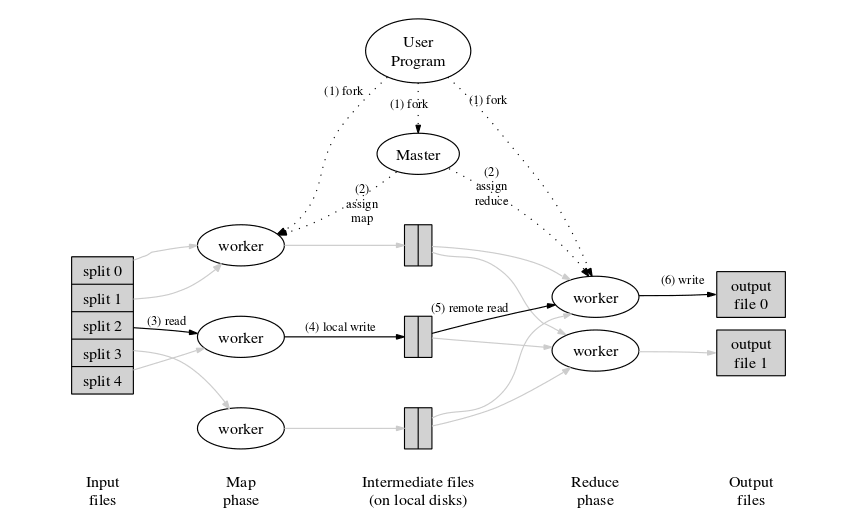
\includegraphics[width=\linewidth]{map-reduce-overview}
  \caption[MapReduce编程模型]{MapReduce编程模型(摘自Google MapReduce论文\cite{Dean2008})}
  \label{fig:map-reduce-overview}
\end{figure}

MapReduce由Google提出\upcite{Dean2008},最初被设计为用于分布式存储计算机集群,
部署在Google的服务器集群之上,执行大规模网络事务处理任务,如网页检索等,表现出很好的性能。
Apache基金会的Hadoop是分布式存储计算机集群上最著名的MapReduce实现。
L\"ammel使用Haskell语言给MapReduce的语义做了精确描述\upcite{Lammel2008}。

Ranger等\upcite{Ranger2007}在共享内存处理器上实现了MapReduce,名为Phoenix,
为MapReduce模型的处理过程提供了更多可配置选项。Phoenix-2是\upcite{Yoo2009}是Phoenix
的改进实现。

MapReduce也被移植到GPU上。香港科技大学的Bingsheng He等在Nvidia GPU上实现了
Mars\upcite{He2008},这是第一个运行在GPU上的Mapreduce系统。由于当时的GPU不支持
动态内存分配,Mars设计了一轮额外的\texttt{map\_count}阶段与一轮额外的\texttt{reduce\_count}
阶段,这带来了一定的附加开销。

MapCG\upcite{Hong2010}是MapReduce系统在GPU上另一版实现。MapCG的贡献是,
统一了MapReduce在CPU端与GPU端的接口设计,并在GPU上实现了一个轻量的动态内存分配器,
从而避免了Mars插入额外处理的开销。

Fang\upcite{Fang2011}增强了了Mars实现,使Mars可以运行在更多并行硬件之上,包括多核CPU、
Nvidia GPU、AMD GPU等,在同时开发CPU/GPU执行计算任务方面进行了一些尝试,
但并未取得理想效果。

Feng\upcite{Ji2011}与Chen\upcite{Chen2012}就GPU片上共享存储器的利用对MapReduce在GPU上
的实现分别提出了不同的优化措施。

Stuart设计了运行在GPU集群上的MapReduce系统GPMR\upcite{Stuart2011}。
出于性能考虑,GPMR向用户暴露了更多硬件细节。GPMR在\texttt{map}阶段
采用了了流水化的执行方式以重叠计算任务与设备件通信。

%% \section{GPU并行编程技术}\label{sec:gpu-parallel-prog}
%% 本节介绍当前使用最广泛的在GPU上进行通用编程的软件技术。

%% \subsection{CUDA}
%% CUDA架构是Nvidia公司针对自己的GPU提出的并行编程框架。
%% 它的提出对GPU通用编程技术产生了巨大的推动力。

%% CUDA为程序员提供了一个完整的GPU编程框架,将GPU的硬件结构
%% 清晰地展现出来。用户使用CUDA C编写在GPU上执行的程序,通常
%% 称为Kernel。CUDA C是一种对C语言的简单扩展,
%% 增加了若干关键字指定程序的执行位置(CPU还是GPU)、变量
%% 的存储位置(全局存储还是贡献存储),
%% 提供了一些内置变量一边获得某些运行时信息。

%% CUDA采用STMD编程模型,这是一种类似与SPMD的编程模型,
%% 一个Kernel程序被一组线程执行,执行路径一般和线程在组中所处的位置相关。
%% 线程按照层次化组织,grid

%% \subsection{OpenCL}

%% \subsection{OpenACC \& OpenHMPP}
